\seite{}{Räumliche Diskretisierung}\anchorpage{1}{neu7}{7 · Räumliche Diskretisierung partieller Differentialgleichungen}\ey{KAPITEL 7}\ptitle{Räumliche Diskretisierung partieller Differentialgleichungen}
Ein Ende eines Stabes wird heiß, das andere bleibt kühl. Ein einziges Thermometer kann den Wärmestrom zwischen beiden nicht bestimmen. Was ändert sich, wenn wir immer mehr Thermometer im Stab verteilen, und an welcher Stelle im Rechenweg erfordert die feinere Ortsauflösung plötzlich kürzere Zeitschritte?
\subt{Der Weg durch das Kapitel}
{\tblstart\begin{tabularx}{\linewidth}{@{}Yr@{}}\toprule
\hyperlink{abs7-1}{7.1 · Linienmethode und Randbedingungen} & \pagelink{abs7-1}\\[2pt]
\hyperlink{abs7-2}{7.2 · Finite Differenzen und diffusive Zeitskalen} & \pagelink{abs7-2}\\[2pt]
\hyperlink{abs7-3}{7.3 · Finite Volumen und hyperbolischer Transport} & \pagelink{abs7-3}\\[2pt]
\hyperlink{abs7-4}{7.4 · Finite Elemente und schwache Form} & \pagelink{abs7-4}\\[2pt]
\bottomrule\end{tabularx}\par}
\par\vfill{\centering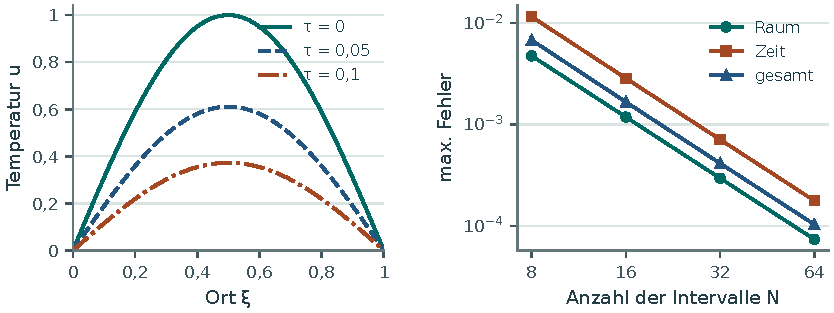
\includegraphics[width=.88\linewidth,height=49mm,keepaspectratio]{mol.pdf}\par}\capline{Nach der Ortsdiskretisierung wird jeder innere Knoten zu einer Zustandskomponente.}
\seite{}{Räumliche Diskretisierung}\anchorpage{2}{abs7-1}{7.1 · Linienmethode und Randbedingungen}\ey{ABSCHNITT 7.1}\ptitle{Linienmethode und Randbedingungen}
\hypertarget{punkt7-1-1}{}\subt{7.1.1\enspace Orts- und Zeitdiskretisierung trennen}
Schneiden wir den Stab in kleine Abschnitte. Jede Temperatur erhält eine Speicherbilanz, jeder Kontakt eine Austauschregel. So entsteht aus \(u_t=\kappa u_{xx}\) nach Wahl der Ortsdiskretisierung das System \(U'=A_hU+b(t)\). Erst jetzt fällt die Wahl des Zeitintegrators. Ein zweiter Versuch mit gleichem Ortsgitter und engeren Zeittoleranzen untersucht gezielt den Zeitfehler.
\hypertarget{punkt7-1-2}{}\subt{7.1.2\enspace Dirichlet, Neumann, Robin und Geisterpunkte}
Ein Bad hält die Randtemperatur fest (Dirichlet), eine Isolierung setzt den Wärmestrom auf null (Neumann), die Kühlung an Luft verknüpft Temperatur und Strom (Robin). Für zentrierte Differenzen an einem Randknoten und \(u_x(0)=0\) folgt aus \((U_1-U_{-1})/(2h)=0\) der Geisterwert \(U_{-1}=U_1\). Am zellzentrierten Rand liegt die Wand eine halbe Zelle entfernt. Dieselbe Indexformel hätte dort eine andere Geometrie.
\seite{Rechenbeispiel}{Räumliche Diskretisierung}\anchorpage{2}{kap6}{Was verraten drei Temperatursensoren?}\ptitle{Was verraten drei Temperatursensoren?}


\lernziel{Sie können eine Temperatur an einem Gitterpunkt fortschreiben, die Einheiten kontrollieren und begründen, warum die räumliche Auflösung den Zeitintegrator beeinflusst.}
Ein Sensor im Innern eines Stabes zeigt \(30\,^\circ\mathrm C\). Ein Zentimeter links davon messen wir \(20\,^\circ\mathrm C\), ein Zentimeter rechts \(24\,^\circ\mathrm C\). Der Heizer ist aus. Wird der mittlere Sensor als Nächstes wärmer oder kälter?
\minifig{dreipunkte}{29mm}{Die Nachbarn sind kälter als die Mitte. Der linke Temperaturunterschied ist größer. Beide Seiten tragen zum Abkühlen der Mitte bei.}
\subt{Was die Nachbarn zur nächsten Steigung beitragen}
Bei konstanter Temperaturleitfähigkeit \(\alpha=0{,}10\unitm{cm^2/s}\) schätzen wir die zweite Ortsableitung durch die Differenz der benachbarten Steigungen. Für die Mitte liefert das
\[
 \dot T_0\approx\alpha\frac{[(24-30)-(30-20)]\unitm K}{(1\unitm{cm})^2}
                 =-1{,}6\unitm{K/s}.
\]
Ein expliziter Euler-Schritt von einer Sekunde ergibt \(28{,}4\,^\circ\mathrm C\). Für alle inneren Punkte gleichzeitig entstehen solche Zeitgleichungen. Genau dieser Übergang von einem räumlichen Feld zu einem System von Zeitgleichungen heißt \emph{Linienmethode}.
\notebox{Vor dem Weiterblättern}{Erhöhen wir alle drei Messwerte um \(5\unitm K\), welche Zahl ändert sich? Die Differenzen und die Steigung bleiben gleich. Nur die neue Temperatur steigt ebenfalls um fünf Kelvin. Eine Rechnung, die jetzt schneller abkühlt, verletzt die angenommene Wärmeleitung.}

\srcs{\textbf{Kernweg}\enspace\see{mol}{Ortsgitter von Hand}\quad\see{molweg}{MOL und Methodenwahl}\quad\see{schwach}{Schwache Form}\quad\see{ueb6}{Selbst prüfen}.}

\lektion{Feld, Randwert und räumliche Ableitung lesen}{feldsprache}{Kernweg}{Felder und Linienmethode}
Eine Messsonde fährt nicht durch den Stab, sie bleibt an ihrem Ort \(x\). Ihre Anzeige im Lauf der Zeit ist \(T(x,t)\) bei festem \(x\). Die Änderung pro Sekunde heißt \(T_t\). Eine Reihe von Sensoren zur gleichen Zeit misst dagegen eine räumliche Steigung \(T_x\) in \(\mathrm{K/m}\). Die Änderung dieser Steigung pro Ortslänge heißt \(T_{xx}\) in \(\mathrm{K/m^2}\). Beim Profil \(T=20+ax^2e^{-bt}\) ergeben sich \(T_x=2ax e^{-bt}\) und \(T_{xx}=2ae^{-bt}\).
\subt{Was wird am Rand vorgegeben?}
Ein \emph{Dirichlet-Rand} schreibt einen Feldwert vor, etwa \(T(0,t)=20\,^\circ\mathrm C\). Ein \emph{Neumann-Rand} schreibt den Normalgradienten bzw. bei bekannter Leitfähigkeit den Fluss vor. Eine isolierte Stirnfläche hat verschwindenden Wärmefluss. Ein \emph{Robin-Rand} verbindet Wert und Fluss, beispielsweise \(-kA T_x(L,t)=G(T(L,t)-T_a)\). Diese Gleichungen beschreiben verschiedene Befestigungen des gleichen Körpers.
\subt{Vom Punkt zum kleinen Volumen}
In mehreren Dimensionen sammelt der \emph{Gradient} \(\nabla T\) alle räumlichen ersten Ableitungen. Die \emph{Divergenz} eines Flusses \(\mathbf j\) ist \(\nabla\cdot\mathbf j=\sum_i\partial j_i/\partial x_i\). Sie misst den lokalen Nettoausfluss pro Volumen. Bei konstanter Leitfähigkeit beschreibt \(\Delta T=\nabla\cdot\nabla T\) die Summe der zweiten Ableitungen. In einer Raumdimension ist das einfach \(T_{xx}\).

Bei Integration über eine Zelle werden die räumlichen Ableitungen zu Randflüssen. In einer Dimension ist das der Hauptsatz \(\int_a^b j_x\dg x=j(b)-j(a)\). In mehreren Dimensionen verknüpft der Gaußsche Integralsatz das Volumenintegral der Divergenz mit dem nach außen gerichteten Fluss durch die Oberfläche. Deshalb kann man im Finite-Volumen-Verfahren jede Zellgrenze genau einmal berechnen und mit entgegengesetzten Vorzeichen verbuchen.
\notebox{Ein Modell ist erst mit seinen Daten bestimmt}{Für die Wärmeleitung im Stab gehören das ganze anfängliche Temperaturprofil und die beiden Randbedingungen zum Problem. Zwei Anfangstemperaturen an den Enden legen die anfängliche Temperatur in der Mitte noch nicht fest.}

\lektion{Aus einer lokalen Bilanz wird ein Feldmodell}{pde}{Kernweg}{Felder und Linienmethode}
\vorhersage{6}{Wir halbieren die Zellbreite bei eindimensionaler Wärmeleitung. Wie ändert sich die Schrittgrenze für nichtnegative Euler-Gewichte?}{kontrolleA}
Schneiden Sie gedanklich ein kurzes Stück \([x,x+\Delta x]\) aus dem Stab. Im Innern speichern Masse und Wärmekapazität ungefähr \(\rho c A\Delta x\,T\) an Energie relativ zu einem festen Bezug. Von links kommt \(q(x)=-kA T_x(x)\), rechts geht \(q(x+\Delta x)\) ab. Hinzu kommt \(P\Delta x/L\) vom Heizer. Teilen durch die Stücklänge und der Grenzübergang liefern die lokale Bilanz
\[
 \rho cA\,T_t=-q_x+P/L=kA\,T_{xx}+P/L .
\]
Jeder Term hat die Einheit Watt pro Meter. Anfangs gilt \(T(x,0)=T_a\). Der isolierte linke Rand liefert \(T_x(0,t)=0\) (Neumann). Rechts liefert die Kontaktkette \(-kA T_x(L,t)=(T(L,t)-T_a)/R\) (Robin). Eine fest vorgegebene Endtemperatur wäre eine Dirichlet-Bedingung.
\subt{Die stationäre Lösung liefert einen unabhängigen Prüfwert}
Im Gleichgewicht gilt \(kA T''=-P/L\). Die linke Randbedingung ergibt \(T'(x)=-Px/(kAL)\). Rechts tritt deshalb genau \(P\) aus. Die Robin-Bedingung liefert \(T(L)=T_a+PR\). Nochmalige Integration ergibt
\[
 T(x)=T_a+PR+\frac{P}{2kAL}(L^2-x^2).
\]
Mit den Daten aus Kapitel 1 sind das \(60{,}00\,^\circ\mathrm C\) am Kontakt zum Stab und \(61{,}25\,^\circ\mathrm C\) an der isolierten Stirnseite. Räumliches Mitteln liefert \(60{,}8333\,^\circ\mathrm C\). Der masselose Zwischenkontakt hat weiterhin \(50\,^\circ\mathrm C\). Alle vier Werte beschreiben verschiedene Messorte oder Mittelungen.
\notebox{Entscheidung}{Gilt am heißen Ende eine zulässige Modellabweichung von \(0{,}5\unitm K\), genügt die Ein-Speicher-Näherung im Dauerbetrieb nicht. Ein beliebig genauer Zeitintegrator für dieses eine Temperaturmodell würde weiterhin \(60\,^\circ\mathrm C\) liefern.}
\srcs{\see{speicher}{Aufwärmkurve des konzentrierten Modells} · \refbk{fnc}{Driscoll und Braun, Linienmethode}.}

\lektion{Die Linienmethode von Hand}{mol}{Kernweg}{Felder und Linienmethode}
Wir richten einen gesonderten Prüfstand für das Ortsgitter ein. Der Heizer wird ausgeschaltet und \emph{beide} Enden werden jetzt auf Umgebungstemperatur gehalten. Mit \(\xi=x/L,\ \tau=\alpha t/L^2,\ \alpha=k/(\rho c)\) und \(u=(T-T_a)/\Delta T\) mit positivem Bezugshub \(\Delta T\) lautet die dimensionslose Wärmegleichung
\[
 u_\tau=u_{\xi\xi},\quad u(0,\tau)=u(1,\tau)=0,\quad
 u(\xi,0)=\sin(\pi\xi).
\]
Einsetzen bestätigt \(u(\xi,\tau)=e^{-\pi^2\tau}\sin(\pi\xi)\). Mit diesen geänderten Randdaten besitzt auch die zeitabhängige Rechnung eine exakte Referenz.
\subt{Erst den Ort diskretisieren}
Auf \(N\) gleich langen Intervallen sei \(\Delta\xi=1/N,\ U_j(\tau)\approx u(j\Delta\xi,\tau)\). Addieren der Taylorreihen um \(\xi_j\) hebt die ungeraden Potenzen auf. Damit ist
\[
 \frac{u(\xi_j-\Delta\xi)-2u(\xi_j)+u(\xi_j+\Delta\xi)}{\Delta\xi^2}
 =u''(\xi_j)+\frac{\Delta\xi^2}{12}u^{(4)}(\xi_j)+O(\Delta\xi^4)
\]
für hinreichend glatte Profile. Die inneren \(N-1\) Werte erfüllen jetzt \(\dot U_j=(U_{j-1}-2U_j+U_{j+1})/\Delta\xi^2\) bei \(U_0=U_N=0\). Die Zeit ist weiterhin kontinuierlich. Diese Trennung heißt Linienmethode (\emph{method of lines}, MOL).
\subt{Dann einen Zeitschritt ausrechnen}
Für vier Intervalle ist \(U(0)=(\sqrt2/2,1,\sqrt2/2)^\mathsf T\). Wir wählen vorwärts Euler mit \(\Delta\tau=0{,}025\), also \(r=\Delta\tau/\Delta\xi^2=0{,}4\). Der mittlere Wert wird zu \(1+0{,}4(\sqrt2-2)=0{,}765685\). Der linke und der rechte Innenwert werden jeweils \(0{,}541421\). Alle liegen zwischen null und eins.
\minifig{gitter4}{25mm}{Vier Intervalle ergeben drei dynamische Innenwerte. Die offene Punktreihe zeigt die Anfangswerte, die Quadrate die drei neuen Werte und die beiden festen Randwerte.}
\notebox{Wo entsteht eine DAE?}{Für den ursprünglichen Stab kann man Flüsse und die unbekannte Kontakttemperatur auf dem Gitter mitführen. Ihre algebraischen Kontaktgleichungen erzeugen Nullzeilen im zeitlichen Massenoperator. Werden sie vorab eliminiert, entsteht hier ein reines ODE-System.}
\srcs{\refbk{fnc}{FNC, The method of lines} · \see{fem}{Massenmatrix bei finiten Elementen}.}

\lektion{Zwei Zellen und ein masseloser Rand}{molrand}{Vertiefung}{Felder und Linienmethode}
Nun kombinieren wir am beheizten Originalstab die Linienmethode mit der algebraischen Kontaktbedingung. Zwei gleich große Kontrollvolumen haben je \(C/2=60\unitm{J/K}\) und erhalten je \(P/2=5\unitm W\). Ihre Temperaturüberschüsse \(U_1,U_2\) sitzen in den Zellzentren. Zwischen den Zentren ergibt Fourier \(q_{12}=(U_1-U_2)/R_{12}\) mit \(R_{12}=\Delta x/(kA)=0{,}125\unitm{K/W}\).

Rechts liegt vom zweiten Zentrum bis zur Stirnfläche noch eine halbe Zelle. Ihr Wärmewiderstand ist \(R_h=\Delta x/(2kA)=0{,}0625\unitm{K/W}\). Damit entsteht die semidiskrete DAE
\[
 \begin{aligned}
 60\dot U_1&=5-q_{12},& 60\dot U_2&=5+q_{12}-q_R,\\
 U_2-\theta_s&=(R_h+R_1)q_R,& \theta_s&=R_2q_R .
 \end{aligned}
\]
Der Zwischenstrom hebt sich beim Addieren beider Speicherbilanzen auf. Startwerte sind \(U_1=U_2=\theta_s=q_R=0\). Eliminiert man die masselosen Kontaktgrößen, folgt \(q_R=U_2/(R_h+R_1+R_2)=U_2/4{,}0625\). Die verbleibenden zwei Gleichungen sind eine ODE.
\subt{Ein Schritt mit Zahlen}
Nach einem Rückwärts-Euler-Schritt von \(60\unitm s\) folgt
\[
 \begin{bmatrix}9&-8\\-8&9+1/4{,}0625\end{bmatrix}
 \begin{bmatrix}U_1\\U_2\end{bmatrix}=\begin{bmatrix}5\\5\end{bmatrix}.
\]
Einsetzen liefert \(U_1=4{,}48759\unitm K,\ U_2=4{,}42354\unitm K\) und \(q_R=1{,}08887\unitm W\). Der rechte Zellmittelpunkt ist kälter, wie die einseitige Kühlung erwarten lässt. Die Speicher nehmen zusammen \(8{,}91113\unitm W\) auf. Mit dem Randstrom sind dies die zugeführten \(10\unitm W\), bis auf Rundung.
\notebox{Modellentscheidung im Detail}{MOL legt hier die räumliche Darstellung fest, die Zeitschrittformel setzt den Zeitfehler. Die Entscheidung, am Rand \(q_R,\theta_s\) gemeinsam zu lösen oder explizit einzusetzen, verändert die Solver-Schnittstelle. Die eliminierte und die simultan gelöste diskrete Form liefern bei exakter linearer Lösung dieselben Temperaturen.}

\lektion{Welche Entscheidung trifft die Linienmethode?}{molweg}{Methodenwahl}{Vom Feld zum Solver}
\textbf{Auftrag.} Für einen dünnen Stab sollen die Temperaturen in der Mitte und nahe dem rechten Ende als Funktion der Zeit berechnet werden. In der Feldgleichung \(T_t=\alpha T_{xx}\) bezeichnet \(T(x,t)\) noch eine Temperatur an jedem Ort und zu jeder Zeit.
\subt{Was übergeben wir an den Zeitintegrator?}
Wählen wir drei gleich weit entfernte innere Messorte und halten beide Enden bei \(0\,^{\circ}\mathrm C\), so wird aus dem Feld ein Vektor \(U=(T_1,T_2,T_3)^\top\). Die \emph{method of lines} (MOL, Linienmethode) ersetzt die räumlichen Ableitungen. An jedem festen Ort bleibt eine stetige Zeitvariable. Für zentrale Differenzen ergibt sich
\[
 \dot U=\frac{\alpha}{\Delta x^2}
 \begin{pmatrix}-2&1&0\\1&-2&1\\0&1&-2\end{pmatrix}U.
\]
Bei \(U=(0,10,0)^\top\,\mathrm K\) als Überschuss und \(\alpha/\Delta x^2=0{,}1\,\mathrm{s}^{-1}\) liefert die Modellfunktion \((1,-2,1)^\top\,\mathrm{K/s}\). Erst Euler etwa mit \(h=1\,\mathrm s\) erzeugt den nächsten Zustand \((1,8,1)^\top\,\mathrm K\).
\subt{Andere Raumdarstellungen führen zur selben Zeitfrage}
{\tblstart\begin{tabularx}{\linewidth}{@{}P{27mm}YY@{}}\toprule
\hd{Raumverfahren}&\hd{Was wird gespeichert?}&\hd{Woran prüfe ich das Ergebnis?}\\\midrule
Differenzen&Knotenwerte. Steigungen aus Nachbarn.&Fehlerabnahme bei Gitterverfeinerung.\\
Finite Volumen&Zellmittelwerte. Flüsse über gemeinsame Flächen.&Zu- und Abfluss jeder Zelle.\\
Finite Elemente&Koeffizienten lokaler Basisfunktionen in der schwachen Form.&Randbedingungen, Energie und Gitterfehler.\\
Spektralverfahren&Koeffizienten globaler Moden.&Abklingen hoher Moden bei glatten Daten.\\\bottomrule
\end{tabularx}\par}
Mit finiten Elementen entsteht oft \(M\dot U=r(t,U)\). Ist die Massenmatrix \(M\) invertierbar, ergibt das Lösen eines linearen Systems die Rate. Bleibt ein masseloser Rand als algebraische Unbekannte erhalten, gehören eine Nebenbedingung und passende Anfangswerte zum DAE-Problem.
\srcs{\href{https://fncbook.com/methodlines/}{Driscoll und Braun, Method of Lines} · \see{molrand}{Ein Rand mit algebraischer Bindung} · \see{schwach}{Schwache Form}.}

\lektion{Parabolisch, hyperbolisch oder elliptisch?}{pdearten}{Kernweg}{Felder und Linienmethode}
Der stationäre Temperaturverlauf des Stabs und seine Aufheizkurve haben verschiedene mathematische Strukturen. Auch die Ausbreitung eines Signals kann ein Feldmodell verlangen. Für die folgenden klassischen Prototypen gibt die Physik den ersten Hinweis.
{\tblstart\begin{tabularx}{\linewidth}{@{}P{27mm}Y@{}}\toprule
\hd{Prototyp}&\hd{Daten, Verhalten und numerische Folge}\\\midrule
Diffusion, parabolisch \(u_t=\alpha u_{xx}\)&Anfangsprofil und passende Randdaten. Kurze Wellen klingen besonders schnell ab. Nach MOL wächst der Betrag des schnellsten Eigenwerts wie \(\Delta x^{-2}\).\\
Welle, hyperbolisch \(u_{tt}=a^2u_{xx}\)&Auslenkung und Geschwindigkeit zu Beginn, dazu passende Randbedingungen. Signale laufen mit endlicher Geschwindigkeit. Phasengang und Energie sind Prüfgrößen.\\
Poisson, elliptisch \(-\nabla\cdot(k\nabla u)=f\)&Randwertproblem im Raum. Eine stationäre Temperatur braucht keine physikalische Anfangszeit. Nach der Diskretisierung wird ein algebraisches Gleichungssystem gelöst.\\\bottomrule
\end{tabularx}\par}
\subt{Ein Netzgleichgewicht konkret lösen}
Beim Stab im Dauerbetrieb verschwindet die Speicherrate. In der FEM-Darstellung bleibt \(KU=b\). Als Beispiel genüge ein lineares Element über die gesamte Länge. Sein Wärmeleitwert beträgt \(kA/L=4\unitm{W/K}\), bei \(k=200\unitm{W/(m\,K)}\) als Wärmeleitfähigkeit des Materials. Bei doppelter Länge und unverändertem Querschnitt beträgt der Leitwert \(2\unitm{W/K}\). Mit \(G=0{,}25\unitm{W/K}\) und gleich verteilter Leistung \(P=10\unitm W\) entsteht
\[
 \begin{bmatrix}4&-4\\-4&4{,}25\end{bmatrix}
 \begin{bmatrix}\theta_0\\ \theta_L\end{bmatrix}
 =\begin{bmatrix}5\\5\end{bmatrix}.
\]
Addition der Zeilen liefert \(0{,}25\theta_L=10\). Rückeinsetzen gibt \(\theta_0=41{,}25\unitm K,\ \theta_L=40\unitm K\). Beide Knotenwerte treffen hier die exakte Lösung. Dazwischen verbindet das Element sie linear, während das exakte Profil quadratisch ist. Ein Vergleich allein an den Randknoten übersieht den Fehler im Inneren.
\notebox{Alternative zum Zeitmarsch}{Bei einer positiv definiten stationären Matrix passen Cholesky oder vorkonditionierte konjugierte Gradienten. Ein rein isolierter Stab mit positiver dauernder Heizleistung besitzt kein stationäres Gleichgewicht. Eine Verträglichkeitsprüfung gehört vor die Wahl des Lösers.}

\seite{}{Räumliche Diskretisierung}\anchorpage{2}{abs7-2}{7.2 · Finite Differenzen und diffusive Zeitskalen}\ey{ABSCHNITT 7.2}\ptitle{Finite Differenzen und diffusive Zeitskalen}
\hypertarget{punkt7-2-1}{}\subt{7.2.1\enspace Der zentrale Diffusionsoperator}
Die Flüsse von links und rechts unterscheiden sich um eine weitere Differenz. Für den inneren Punkt gilt \(U'_j=\kappa(U_{j-1}-2U_j+U_{j+1})/h_x^2\). Einsetzen eines konstanten Profils ergibt null. Einsetzen von \(x^2\) ergibt exakt \(2\kappa\). Die Taylor-Reste der Nachbarn zeigen für glatte Profile einen Ortsfehler zweiter Ordnung.
\hypertarget{punkt7-2-2}{}\subt{7.2.2\enspace Warum Halbieren des Gitters vier Schritte kostet}
Der alternierende Gittermodus \((1,-1,1,-1,\ldots)\) trägt auf dem periodischen geraden Gitter den Eigenwert \(-4\kappa/h_x^2\). Damit fordert Vorwärts-Euler \(h_t\le h_x^2/(2\kappa)\). Halbiert man \(h_x\), vervierfacht sich die Zahl der Zeitschritte auf demselben Intervall. Ein impliziter Integrator kann diese Stabilitätsgrenze überwinden. Die räumliche Genauigkeit und das Budget für die linearen Lösungen bleiben zu prüfen.
\lektion{Warum ein feineres Gitter steifer wird}{gitterstabil}{Kernweg}{Felder und Linienmethode}
Wie groß darf ein Zeitschritt sein, wenn keine neue heißeste oder kälteste Stelle entstehen soll? Sammeln wir am Innenknoten alle Koeffizienten der alten Temperaturen. Der explizite Diffusionsschritt lautet
\[
 U_j^{n+1}=rU_{j-1}^n+(1-2r)U_j^n+rU_{j+1}^n .
\]
Für \(0\le r\le1/2\) sind alle Gewichte nichtnegativ und addieren sich zu eins. Jeder neue Wert liegt damit im Bereich seiner Nachbarn einschließlich des eigenen alten Werts. Per Induktion bleiben die globalen Extremwerte bei homogenen Dirichlet-Rändern durch die Extremwerte aus Start und Rand beschränkt. Das ist das diskrete Maximumprinzip.
\subt{Beweis der spektralen Schranke}
Die Gitterfunktion \(v_j=\sin(k\pi j/N)\) verschwindet an beiden Enden. Aus \(\sin(a-b)+\sin(a+b)=2\sin(a)\cos(b)\) folgt
\[
 (D_{xx}v)_j=\lambda_k v_j,\qquad
 \lambda_k=-4N^2\sin^2\!\left(\frac{k\pi}{2N}\right),\quad 1\le k<N.
\]
Die Sinusmoden bilden eine orthogonale Basis. Jede Amplitude wird durch Euler mit \(1+\Delta\tau\lambda_k\) multipliziert. Die größtmögliche Frequenz \(k=N-1\) bestimmt deshalb die exakte Stabilitätsgrenze in der euklidischen Norm:
\[
 r\le\frac{1}{2\cos^2(\pi/(2N))}.
\]
Für ein endliches Gitter liegt sie geringfügig über \(1/2\). Die einfachere Schranke \(r\le1/2\) sichert zusätzlich das Maximumprinzip. Wenn \(\Delta\xi\) halbiert wird, muss für diese explizite Bedingung \(\Delta\tau\) geviertelt werden.
\subt{Was ein impliziter Schritt ändert}
Bei rückwärts Euler wird \((I-\Delta\tau D_{xx})U^{n+1}=U^n\) gelöst. Die Matrix ist tridiagonal. Radau und BDF können dieselbe lokale Kopplungsstruktur nutzen. Die implizite Dämpfung befreit von der obigen linearen Euler-Schranke. Soll gerade der Abbau einer schnellen Mode genau aufgelöst werden, bleibt ihre Zeitskala wichtig.
\task{4}{Für \(\alpha=10^{-4}\,\mathrm{m^2/s}\) und \(\Delta x=2\unitm{cm}\) bestimmen Sie einen maximalen Euler-Schritt nach dem Maximumprinzip. Was gilt bei halbem Gitterabstand?}

\lektion{Raum- und Zeitfehler einzeln messen}{raumfehler}{Kernweg}{Felder und Linienmethode}
Wir beobachten den sinusförmigen Prüfstand bei \(\tau_f=0{,}1\). Die PDE liefert \(u^*(\xi)=e^{-\pi^2\tau_f}\sin(\pi\xi)\). Für jedes Gitter kennen wir außerdem die \emph{exakte Lösung des räumlich diskreten Systems}, \(U_j^h=e^{\lambda_1\tau_f}\sin(\pi j/N)\). Schließlich berechnet vorwärts Euler \(U_j^{h,k}\) bei \(r=0{,}4\). Damit stehen zwei unabhängige Vergleiche zur Verfügung.
{\tblstart\begin{tabularx}{\linewidth}{@{}rrYYY@{}}\toprule
\hd{\(N\)}&\hd{Schritte}&\hd{Raumfehler}&\hd{Zeitfehler}&\hd{Gesamtfehler}\\\midrule
8&16&\(4{,}733\cdot10^{-3}\)&\(1{,}150\cdot10^{-2}\)&\(6{,}762\cdot10^{-3}\)\\
16&64&\(1{,}182\cdot10^{-3}\)&\(2{,}846\cdot10^{-3}\)&\(1{,}663\cdot10^{-3}\)\\
32&256&\(2{,}955\cdot10^{-4}\)&\(7{,}097\cdot10^{-4}\)&\(4{,}142\cdot10^{-4}\)\\
64&1024&\(7{,}386\cdot10^{-5}\)&\(1{,}773\cdot10^{-4}\)&\(1{,}034\cdot10^{-4}\)\\\bottomrule
\end{tabularx}\par}
\capline{Maximumnorm über alle inneren Knoten. Raumfehler \(\|U^h-u^*\|_\infty\), Zeitfehler \(\|U^{h,k}-U^h\|_\infty\), Gesamtfehler \(\|U^{h,k}-u^*\|_\infty\).}
\fig{mol}{.95}{Links bleibt die Form der Grundmode erhalten. Rechts sinken die Fehler bei Gitterverdopplung etwa auf ein Viertel. Hier wird gleichzeitig der Zeitschritt geviertelt.}
\subt{Weshalb der Gesamtfehler kleiner als der Zeitfehler ist}
Für die Grundmode ist \(|\lambda_1|<\pi^2\), das Ortsgitter dämpft also zu schwach. Euler dämpft diese Mode im gewählten Bereich zu stark, denn \(0<1+z<e^z\) bei \(-1<z<0\). Die Fehler wirken gegeneinander. Aus dem Gesamtfehler allein ließe sich diese Kompensation nicht erkennen. Die beobachtete Ordnung nahe zwei gegenüber \(\Delta\xi\) ist mit dem Zeitfehler erster Ordnung bei \(\Delta\tau=0{,}4\Delta\xi^2\) vereinbar.
\srcs{Eigener Rechenversuch · expliziter Dreipunktoperator in \texttt{molexperiment}, gegengeprüft mit der analytischen Verstärkung jeder Rechnung.}

\lektion{Ein Energiebeweis für die Wärmegleichung}{waermebeweis}{Vertiefung}{Felder und Linienmethode}
Könnten zwei verschiedene Temperaturfelder dieselbe Geometrie, Heizleistung, Anfangstemperatur und Randbedingung erfüllen? Für hinreichend glatte Lösungen \(T_1,T_2\) betrachten wir ihre Differenz \(w=T_1-T_2\). Die Quelle fällt heraus. Links bleibt \(w_x(0,t)=0\), rechts \(-kAw_x(L,t)=G w(L,t)\) mit \(G=1/R>0\).
\subt{Satz · Eindeutigkeit bei gekühltem Rand}
Zwei solche Lösungen mit gleichem Anfangsprofil stimmen im gesamten Zeitintervall überein.
\proofpart{Multipliziere \(\rho c A w_t=kA w_{xx}\) mit \(w\) und integriere über den Stab. Für das nichtnegative quadratische Funktional \(\mathcal E=\frac12\int_0^L \rho c A w^2\dg x\) folgt durch partielle Integration
\[
 \dot{\mathcal E}
  = kA[ww_x]_0^L-kA\int_0^L w_x^2\dg x
  =-G w(L,t)^2-kA\int_0^L w_x^2\dg x\le0 .
\]
Bei gleichen Anfangsdaten ist \(\mathcal E(0)=0\). Das Funktional bleibt zugleich nichtnegativ und höchstens null. Daher ist \(w=0\) und wegen der angenommenen Stetigkeit sind beide Felder überall gleich.}
\subt{Wie man den Beweis im Code nutzt}
Für zwei Lösungen des linearen FEM-Systems bei gleichem Eingang erfüllt der Differenzvektor \(W\) die Gleichung \(M\dot W+KW=0\). Damit folgt \(\dd(W^\mathsf TMW/2)/\dd t=-W^\mathsf TKW\le0\). Ein Test kann zufällige Gittervektoren einsetzen und die Vorzeichen der beiden quadratischen Formen prüfen. Eine falsche Orientierung am Robin-Rand verändert genau den Randterm dieses Beweises.

Dieses Funktional misst die quadratische Abweichung zweier Temperaturfelder. Die physikalische Wärmebilanz des Originalstabs verwendet dagegen \(\int_0^L \rho c A(T-T_a)\dg x\); sie ist linear in der Temperaturdifferenz. Ein Solver sollte beide Strukturen entsprechend dem jeweiligen Versuch abbilden.
\srcs{\see{pde}{Kontinuierliche Bilanz} · \see{fem}{schwache Form und Massenmatrix} · \see{lyapunov}{mechanische Energiebilanz}.}

\lektion{Transport explizit, Diffusion implizit?}{imex}{Vertiefung}{Felder und Linienmethode}
In einer geraden Leitung mit konstanter Geschwindigkeit \(a>0\) und Dispersion \(D>0\) ist der Gesamtfluss \(ac-Dc_x\). Die Stoffbilanz ergibt \(c_t+ac_x=Dc_{xx}\). Wir betrachten ein periodisches Gitter, um Randfehler auszuschließen. Das Feld werde durch Zellmittel dargestellt. Für den nach rechts gerichteten Transport wählen wir den Aufwindfluss, für die Diffusion eine zentrale Differenz des Gradienten.
\subt{Zwei Schranken wirken im selben Schritt}
Der vollständig explizite Euler-Schritt lässt sich schreiben als
\[
 c_j^{n+1}=(\nu+r)c_{j-1}^n+(1-\nu-2r)c_j^n+r c_{j+1}^n,\qquad
 \nu=\frac{a h}{\Delta x},\quad r=\frac{Dh}{\Delta x^2}.
\]
Die Gewichte addieren sich zu eins. Eine konvexe Kombination entsteht für \(\nu+2r\le1\). Bei \(a=1\unitm{m/s},\ D=0{,}01\unitm{m^2/s}\) und \(\Delta x=0{,}01\unitm m\) folgt \(h\le1/300\unitm s\). Die isolierten Einzelgrenzen wären \(0{,}01\unitm s\) und \(0{,}005\unitm s\). Selbst deren Minimum macht den mittleren Koeffizienten im gemeinsamen expliziten Schritt bereits negativ.
\subt{IMEX · Eine Schrittformel, zwei Behandlungen}
Bezeichne \(A_h\) den räumlichen Advektionsoperator und \(D_h\) den räumlichen Diffusionsoperator. Ein IMEX-Euler-Schritt lautet
\[
 (I-hD_h)c^{n+1}=c^n+hA_h c^n .
\]
Bei \(\nu\le1\) ist die rechte Seite ein nichtnegatives Gemisch der alten Zellen. Der implizite Diffusionsschritt erhält hier die Nichtnegativität: Wäre der kleinste neue Wert negativ, ergäbe die zugehörige Zeile von \((I-hD_h)c^{n+1}\) höchstens diesen negativen Wert. Das widerspricht einer nichtnegativen rechten Seite. Im Beispiel sind so Schritte bis \(0{,}01\unitm s\) unter diesem Kriterium möglich. Die Zeitgenauigkeit bleibt erster Ordnung.
\subt{Alternative · Operatoraufspaltung}
Bei der Strang-Aufspaltung folgen eine halbe Diffusionsphase, eine volle Transportphase und eine halbe Diffusionsphase. Bei glatten Lösungen und hinreichend genauen Teilflüssen ist die Zusammensetzung unter den üblichen Regularitätsbedingungen zweiter Ordnung. Für konstante Koeffizienten und die hier gewählten periodischen Operatoren kommutieren die Matrizen. Bei exakten Teilflüssen verschwindet dann der reine Aufspaltungsfehler. Variable Koeffizienten und Ränder erfordern eine neue Prüfung.
\srcs{\href{https://doi.org/10.1016/S0168-9274(97)00056-1}{Ascher, Ruuth und Spiteri, IMEX} · \href{https://doi.org/10.1137/0705041}{Strang, Operatoraufspaltung} · \see{c19}{Advektion und Dispersion bei C19R}.}

\seite{}{Räumliche Diskretisierung}\anchorpage{2}{abs7-3}{7.3 · Finite Volumen und hyperbolischer Transport}\ey{ABSCHNITT 7.3}\ptitle{Finite Volumen und hyperbolischer Transport}
\hypertarget{punkt7-3-1}{}\subt{7.3.1\enspace Eine Grenzfläche, ein gemeinsamer Fluss}
Ein Wasserpaket, das die rechte Seite einer Zelle verlässt, tritt links in die Nachbarzelle ein. Mit Zellmittelwerten gilt \(\bar u_j^{n+1}=\bar u_j^n-\Delta t(F_{j+1/2}-F_{j-1/2})/\Delta x\). Beim Aufsummieren heben sich alle inneren Flüsse paarweise auf. Randflüsse und Quellen bestimmen die globale Bilanz.
\hypertarget{punkt7-3-2}{}\subt{7.3.2\enspace Upwind, zentrale Approximation und Wellenform}
Für \(f(u)=au,\ a>0\) nimmt Upwind den linken Zustand am Übergang. Der Update \((1-C)u_j+Cu_{j-1}\) ist bei \(0\le C=a\Delta t/\Delta x\le1\) eine konvexe Mischung. Ein scharfer Sprung verschmiert. Eine zentrale Ortsableitung mit Vorwärts-Euler ist für lineare Advektion instabil. Zentrierte Verfahren mit geeigneter Zeitdiskretisierung können stattdessen dispersive Über- und Unterschwinger zeigen.
\hypertarget{punkt7-3-3}{}\subt{7.3.3\enspace TVD, Minmod und Superbee}
Die diskrete Gesamtvariation lautet \(TV(u)=\sum_j|u_{j+1}-u_j|\). Ein TVD-Schritt vergrößert sie unter seinen CFL- und Randannahmen nicht. Minmod setzt gegensinnige Steigungen auf null und wählt bei gleichem Vorzeichen die betragskleinere. Für das Steigungsverhältnis \(r\) gilt \(\phi_{MM}=\max(0,\min(1,r))\) und \(\phi_{SB}=\max(0,\min(2r,1),\min(r,2))\). Superbee lässt steilere Fronten zu. Eine konstante Nachbarschaft muss die Implementierung ohne Division durch null behandeln.
\lektion{Finite Volumen und Charakteristiken für Transport}{fvm}{Kernweg}{Felder und Linienmethode}
Ein Stoff mit Konzentration \(c(x,t)\) bewegt sich in einer geraden Leitung mit konstanter Geschwindigkeit \(a>0\). Querschnitt, Dichte und Geschwindigkeit seien konstant. Reaktion und Diffusion fehlen. Die Stoffmenge einer Zelle ändert sich genau um Zufluss minus Abfluss. Das führt auf \(c_t+(ac)_x=0\). Am Eintritt ist die Konzentration vorzugeben. Bei reinem Transport nach rechts benötigt der Austritt keine zusätzliche Konzentrationsbedingung.
\subt{Zellmittel und gemeinsame Flüsse}
Für Zellmittel \(\bar c_j\) folgt durch Integration über eine Zelle
\[
 \dot{\bar c}_j=-\frac{F_{j+1/2}-F_{j-1/2}}{\Delta x}.
\]
Der Aufwindfluss \(F_{j+1/2}=a\bar c_j\) übernimmt die Konzentration stromaufwärts. Summiert man die Gleichung über alle Zellen, heben sich alle inneren Flüsse paarweise auf. Die Gesamtmenge ändert sich nur durch die beiden äußeren Flüsse. Dieser Erhaltungsbeweis gilt für jeden gemeinsamen numerischen Fluss.

Mit vorwärts Euler lautet der Schritt \(\bar c_j^{n+1}=(1-\nu)\bar c_j^n+\nu\bar c_{j-1}^n,\quad\nu=a\Delta t/\Delta x\). Bei \(a=2\unitm{m/s},\ \Delta x=0{,}04\unitm m\) folgt \(\Delta t\le0{,}02\unitm s\) aus \(0\le\nu\le1\). Bei \(\nu=1\) rückt jedes Zellmittel exakt um eine Zelle weiter. Bei \(\nu=1/2\) wird eine Sprungfront auf Nachbarzellen verteilt.
\subt{Eine alternative Rechnung entlang der Bewegung}
Entlang \(x(t)=x_0+at\) gilt \(\dd c(x(t),t)/\dd t=c_t+ac_x=0\). Diese Charakteristik liefert die exakte Lösung als verschobenes Anfangsprofil, bis eine vom Einlass eintreffende Information die Stelle erreicht. Semi-Lagrange-Verfahren verfolgen eine Charakteristik rückwärts und interpolieren am Fußpunkt. Konservative Varianten benötigen eine entsprechende Fluss- oder Rekonstruktionsvorschrift.
\notebox{Methodenwahl}{Bei scharfen Fronten und einer Mengenbilanz ist ein konservatives Finite-Volumen-Verfahren mit geeignetem Fluss und Begrenzer naheliegend. Bei einem glatten Wärmefeld auf einem regelmäßigen Gitter genügt oft schon die zentrale finite Differenz.}
\srcs{\refbk{fv}{LeVeque, Finite Volume Methods for Hyperbolic Problems}.}

\lektion{Kann ein erhaltendes Verfahren negative Werte liefern?}{laxtransport}{Rechenversuch}{Transport}
Markierstoff bewegt sich in einem periodischen Kanal mit konstanter Geschwindigkeit \(a>0\). Vier gleich große Zellen enthalten anfangs die normierten Mittelwerte \((0,1,1,0)\). Während eines Schritts bewegt sich das Profil um eine halbe Zelle. Die dimensionslose Courant-Zahl ist damit \(C=ah/\Delta x=1/2\). Die linke Nachbarin von Zelle 1 ist Zelle 4.
\subt{Zwei Regeln, dieselben Daten}
Das Upwind-Verfahren nimmt den zufließenden Wert von links. Lax--Wendroff berücksichtigt zusätzlich die Krümmung aus beiden Nachbarn. Für die lineare Transportgleichung \(u_t+a u_x=0\) lauten beide vollständig diskreten Regeln
\begin{align*}
 U_j^{n+1}&=U_j^n-C(U_j^n-U_{j-1}^n),\\
 V_j^{n+1}&=V_j^n-\tfrac C2(V_{j+1}^n-V_{j-1}^n)
             +\tfrac{C^2}2(V_{j+1}^n-2V_j^n+V_{j-1}^n).
\end{align*}
{\tblstart\begin{tabularx}{\linewidth}{@{}Yrrrrr@{}}\toprule
\hd{Nach einem Schritt}&\hd{Zelle 1}&\hd{2}&\hd{3}&\hd{4}&\hd{Summe}\\\midrule
Upwind&0&0,5&1&0,5&2\\
Lax--Wendroff&$-0{,}125$&0,625&1,125&0,375&2\\\bottomrule
\end{tabularx}\par}
In Zelle 1 ist die Konzentration nach Lax--Wendroff negativ. Eine höhere Genauigkeitsordnung für glatte Daten beantwortet die Frage nach Positivität an einem Sprung also noch nicht. In diesem einen Schritt liefert Upwind sogar die exakten Zellmittel des um eine halbe Zelle verschobenen, ursprünglich stückweise konstanten Profils. Wiederholtes Mitteln verbreitert die Front.
\subt{Was können wir für beliebige Eingaben beweisen?}
\proofpart{Upwind bildet bei \(0\le C\le1\) die konvexe Kombination \((1-C)U_j+C U_{j-1}\). Sie liegt zwischen den Nachbarwerten. Bei periodischer Summation heben sich in beiden Regeln alle Differenzen auf. Beide erhalten daher die Gesamtmenge \(\Delta x\sum_j U_j\).}
\srcs{\href{https://www.clawpack.org/fvmhp_materials/}{LeVeque, Finite Volume Methods for Hyperbolic Problems} · \texttt{python methodenlabor.py} · \see{schluss6}{Fragen zur Methodenwahl}.}

\seite{}{Räumliche Diskretisierung}\anchorpage{2}{abs7-4}{7.4 · Finite Elemente und schwache Form}\ey{ABSCHNITT 7.4}\ptitle{Finite Elemente und schwache Form}
\hypertarget{punkt7-4-1}{}\subt{7.4.1\enspace Von der Wärmebilanz zur Galerkin-Projektion}
Multipliziert man \(u_t=\kappa u_{xx}\) mit einer Testfunktion \(v\) und integriert partiell, entsteht \(\int v u_t+\int \kappa v_xu_x=[v\kappa u_x]_{\partial\Omega}\). Für die Ortsanteile genügen quadratintegrable Funktionen mit quadratintegrabler schwacher erster Ableitung, der Sobolev-Raum \(H^1\). Vorgegebene Dirichlet-Werte schränken den Lösungsraum ein, die zugehörigen Testfunktionen verschwinden dort.
\hypertarget{punkt7-4-2}{}\subt{7.4.2\enspace Massen- und Steifigkeitsmatrix}
Im Ansatz \(u_h=\sum_j U_j\varphi_j\) wählt Galerkin \(v=\varphi_i\). Somit gilt \(M\dot U+KU=b\), mit \(M_{ij}=\int\varphi_i\varphi_j\) und \(K_{ij}=\int\kappa\varphi'_i\varphi'_j\). Die Hutfunktionen überlappen nur Nachbarn, weshalb beide Matrizen dünn besetzt sind. Eine reguläre Massenmatrix liefert ein ODE-System. Zusätzliche Multiplikatoren oder masselose Freiheitsgrade können eine DAE erzeugen.

Auf einem einzigen Element der Länge \(\ell\) lässt sich jeder Eintrag ausrechnen. Mit \(\xi=x/\ell\) fallen und steigen die beiden Hutfunktionen als \(1-\xi\) und \(\xi\). Daher ist \(M_{11}=\ell\int_0^1(1-\xi)^2\,\mathrm d\xi=\ell/3\) und \(M_{12}=\ell\int_0^1(1-\xi)\xi\,\mathrm d\xi=\ell/6\). Die räumlichen Ableitungen sind konstant \(-1/\ell\) und \(1/\ell\). Für eine konstante Diffusivität \(\kappa\) folgt
\[
 M_e=\frac{\ell}{6}\begin{pmatrix}2&1\\1&2\end{pmatrix},\qquad
 K_e=\frac{\kappa}{\ell}\begin{pmatrix}1&-1\\-1&1\end{pmatrix}.
\]
Beim Zusammenbau werden die Beiträge beider angrenzenden Elemente am gemeinsamen Knoten addiert. Eine konstante Temperatur ohne Randantrieb muss die Steifigkeitsmatrix auf null abbilden. Genau das zeigen die verschwindenden Zeilensummen von \(K_e\).
\lektion{Vier Raumverfahren an einem warmen Mittelpunkt}{raumwahl}{Kernweg}{Felder und Linienmethode}
Ein dimensionsloser Stab reicht von 0 bis 1. Beide Enden bleiben bei null, die anfängliche Temperatur ist \(u(\xi,0)=\sin(\pi\xi)\). Für \(u_\tau=u_{\xi\xi}\) schätzen wir, wie schnell die Temperatur an der Mitte fällt. Ein sehr grobes Gitter hat nur den inneren Wert \(U(0)=1\) zwischen zwei Randwerten null. Was ändert sich, wenn wir den Ort verschieden beschreiben?
\subt{Differenzen und Volumen liefern hier dieselben Zahlen}
Bei \(\Delta\xi=1/2\) ergibt die zweite Differenz \((0-2U+0)/(1/2)^2=-8U\). Nehmen wir stattdessen ein \emph{knotenzentriertes Kontrollvolumen} von der Stelle \(1/4\) bis \(3/4\), fließen bei linear angenäherten Randgradienten links \(2U\) und rechts \(2U\) hinaus. Der Inhalt ist näherungsweise \(U/2\). Seine Bilanz \(\dot U/2=-4U\) liefert wiederum \(-8U\). Der Punkt über \(U\) bezeichnet hier die Ableitung nach \(\tau\).
\subt{Was die übrigen Darstellungen speichern}
Bei linearen finiten Elementen tragen die beiden Randknoten null. Der einzige freie Koeffizient multipliziert eine Hutfunktion \(\phi\), die in der Mitte eins und an den Rändern null ist. Es gilt \(\int_0^1\phi^2\,\mathrm d\xi=1/3\) und \(\int_0^1(\phi')^2\,\mathrm d\xi=4\). Die Wärmebilanz in schwacher Form liefert also \((1/3)\dot U=-4U\). Eine Spektralmethode kann stattdessen genau die hier vorgegebene Sinusform als Basisfunktion benutzen.
{\tblstart\begin{tabularx}{\linewidth}{@{}Yl@{}}\toprule
\hd{Raumbeschreibung}&\hd{Steigung anfangs in der Mitte}\\\midrule
Finite Differenzen oder obiges Kontrollvolumen&\(-8\)\\
Lineare Elemente mit konsistenter Massenmatrix&\(-12\)\\
Passende Sinusbasis, zugleich exakte Referenz&\(-\pi^2\approx-9{,}87\)\\\bottomrule\end{tabularx}\par}
Die Gittermodelle teilen den Anfangswert am Mittelpunkt, stellen das Anfangsprofil zwischen den Punkten aber verschieden dar. Dieselbe Zeitroutine könnte alle drei Zeitgleichungen integrieren. Der Unterschied entsteht bereits vor deren erstem Schritt.
\srcs{\see{fvm}{Zellflüsse für Transport} · \see{schwach}{Herleitung der schwachen Form} · \see{fem}{Elemente und Spektralverfahren}.}

\lektion{Von der Wärmebilanz zur schwachen Form}{schwach}{Vertiefung}{Felder und Linienmethode}
Zeichnen Sie zwei Geradenstücke, die mit einem Knick zusammentreffen. Am Knick existiert keine gewöhnliche zweite Ableitung. Trotzdem sind solche stückweise linearen Profile für die Temperaturrechnung brauchbar. Dazu übersetzen wir die punktweise Forderung der \emph{starken Form} in eine Bilanz mit weniger Ableitungen.
\subt{Mit einer Testfunktion gewichten}
Betrachten wir stationär \(-kT''=s\) auf \([0,L]\), zunächst mit einer an den Enden verschwindenden glatten Testfunktion \(v\). Multiplikation und Integration ergeben \(-\int_0^L kvT''\dg x=\int_0^L vs\dg x\). Partielle Integration folgt aus der Produktregel \((vT')'=v'T'+vT''\). Der Randterm verschwindet mit \(v\). Somit gilt
\[
 \int_0^L k v'T'\dg x=\int_0^L vs\dg x .
\]
In dieser \emph{schwachen Form} genügt unter dem Integral eine erste Ortsableitung. Sind Randwerte nicht vorgeschrieben, kann ein Randterm verbleiben. Der gekühlte Rand des Stabs auf der folgenden Seite zeigt das konkret.
\subt{Eine Hutfunktion von Hand zeichnen}
Auf drei aufeinanderfolgenden Knoten sei \(\phi\) links null, in der Mitte eins und rechts wieder null. Dazwischen verläuft sie linear, außerhalb ebenfalls null. In einer finiten Elementdarstellung werden solche Formen mit den gesuchten Knotentemperaturen gewichtet und addiert. Als Testfunktion wählen wir nacheinander denselben Satz von Hüten. So entsteht eine Zeile des algebraischen Gleichungssystems pro unabhängigem Knoten.
\subt{Warum eine Matrix positiv sein kann}
Eine reelle symmetrische Matrix \(K\) heißt positiv definit, falls \(w^\mathsf T K w>0\) für jeden \(w\ne0\) gilt. Für solche Matrizen kann eine Cholesky-Zerlegung \(K=LL^\mathsf T\) das lineare System lösen. Das Verfahren der konjugierten Gradienten sucht die Lösung iterativ in aufeinander aufbauenden Richtungen. Eine \emph{Vorkonditionierung} löst dabei ein einfacher handhabbares Hilfssystem, um die Iteration zu beschleunigen. Im Wärmebeispiel verrät die Energiebilanz, unter welchen Randbedingungen die stationäre Matrix diese Positivität besitzt.
\srcs{\refbk{fem}{Dokken, Wärmegleichung und finite Elemente}.}

\lektion{Finite Elemente, Spektralmethoden und Modellklasse}{fem}{Vertiefung}{Felder und Linienmethode}
Beim ursprünglichen Stab ist die Randbedingung eine Wärmeabfuhr über \(R\). Schreibe \(\theta=T-T_a,\ G=1/R\). Multiplikation der PDE mit einer Testfunktion \(v\), Integration über den Stab und partielle Integration des Leitungsflusses ergeben
\[
 \int_0^L \rho cA\,v\,\dot\theta\dg x
 +\int_0^L kA\,v'\theta'\dg x
 +Gv(L)\theta(L)=\int_0^L v\,P/L\dg x .
\]
Der Robin-Term folgt unmittelbar aus der Randbilanz. Mit stückweise linearen Hutfunktionen \(\phi_i\) auf dem Gitter und \(\theta_h=\sum_j U_j\phi_j\) wählt man nacheinander \(v=\phi_i\). Die Elementmatrizen einer Zelle der Länge \(\ell\) sind
\[
 M_e=\frac{\rho cA\ell}{6}\begin{bmatrix}2&1\\1&2\end{bmatrix},\qquad
 K_e=\frac{kA}{\ell}\begin{bmatrix}1&-1\\-1&1\end{bmatrix}.
\]
Auf dem Referenzelement \(0\le s\le1\) sind die Basisfunktionen \(1-s\) und \(s\). Die Integrale \(\int_0^1 s^2\dg s=1/3\) und \(\int_0^1 s(1-s)\dg s=1/6\) erklären die beiden Gewichte der Massenmatrix. Für konstante Heizleistung entfällt pro Element auf jeden Knoten \(P\ell/(2L)\). Beim Zusammenbauen addiert man die Beiträge benachbarter Zellen. \(G\) kommt auf den letzten Diagonaleintrag von \(K\). Es entsteht \(M\dot U+KU=b\). Für jeden von null verschiedenen Koeffizientenvektor \(w\) gilt \(w^\mathsf TMw=\int\rho c A(\sum_iw_i\phi_i)^2\dg x>0\). Somit ist \(M\) invertierbar, die Semidiskretisierung eine ODE.
\subt{Andere Fragen brauchen andere Raumverfahren}
{\tblstart\begin{tabularx}{\linewidth}{@{}P{26mm}Y@{}}\toprule
\hd{Verfahren}&\hd{Was spricht für die Wahl?}\\\midrule
Finite Differenzen&Ein regelmäßiges Gitter und ein glatter Feldverlauf geben einen kurzen, günstigen Differenzenoperator.\\
Finite Volumen&Geteilte Grenzflüsse erhalten die Zellbilanz. Fronten, Ein- und Ausstrom lassen sich direkt prüfen.\\
Finite Elemente&Die schwache Form passt zu unregelmäßigen Geometrien, variablen Stoffwerten und gemischten Randbedingungen.\\
Spektralverfahren&Für glatte, periodische Felder zerlegt eine Fourierbasis lineare Ableitungen in Moden. Sprünge erzeugen Gibbs-Schwingungen.\\\bottomrule
\end{tabularx}\par}
\srcs{\refbk{fem}{Dokken, Wärmegleichung in schwacher Form} · \refbk{fnc}{Driscoll und Braun}.}

\werkblatt{7}{Selbst prüfen}{ueb6}{Nachbarn, Zeitschritt und Erhaltung}

\merke{Nach der räumlichen Diskretisierung trägt jeder innere Gitterpunkt eine Zeitgleichung. Die Kopplungen zwischen den Punkten enthalten die Zellweite und die Physik.}
\subt{A · Eine neue Temperatur berechnen}
Drei benachbarte Gitterwerte eines homogenen Stabes sind \(10,\ 16,\ 14\,^\circ\mathrm C\). Wir untersuchen den mittleren Punkt. Für einen Euler-Schritt betrage \(r=\alpha h/\Delta x^2=0{,}2\). Berechnen Sie die neue Temperatur aus \(T_0^{\rm neu}=T_0+r(T_- -2T_0+T_+)\). Liegt sie zwischen den bisherigen Extremwerten?
\subt{B · Ein feineres Gitter kann ein kälteres Minimum erzeugen}
Die Zellweite wird halbiert, \(h\) bleibt zunächst gleich. Bestimmen Sie das neue \(r\). Prüfen Sie die Werte \(0,\ 10,\ 0\,^\circ\mathrm C\) für einen Schritt. Wie muss \(h\) verändert werden, wenn der ursprüngliche Faktor \(r=0{,}2\) wieder gelten soll?
\subt{C · Erhaltung in einem anderen Raummodell prüfen}
Zwei nach außen isolierte Körper mit \(C_1=2\unitm{J/K}\) und \(C_2=1\unitm{J/K}\) sind durch einen Wärmeleitwert \(G=1\unitm{W/K}\) verbunden. Sie starten bei \(20\) und \(14\,^\circ\mathrm C\). Bestimmen Sie die beiden Anfangssteigungen und die gemeinsame Endtemperatur. Welche gewichtete Summe muss Ihr Code während der Rechnung erhalten?
\hilfe{In C erhält ein Körper genau die Leistung, die der andere verliert. Temperatursummen ohne die zugehörigen Wärmekapazitäten haben diese Eigenschaft im Allgemeinen nicht.}

\schreibfeld

\srcs{\see{loesweg6}{Lösungswege A, B und C}\quad·\quad\see{kap6}{Zum Kapitelauftakt}.}

\werkblatt{7}{Lösungswege}{loesweg6}{Nachbarn, Zeitschritt und Erhaltung}

\subt{A · Den neuen Wert einordnen}
Die zweite Differenz ist \(10-2\cdot16+14=-8\unitm K\). Der neue Wert beträgt \(16-0{,}2\cdot8=14{,}4\,^\circ\mathrm C\). Er liegt zwischen 10 und 16 Grad. Man kann die Vorschrift auch als \(0{,}2T_-+0{,}6T_0+0{,}2T_+\) lesen. Die nichtnegativen Gewichte summieren sich zu eins, also kann dieser Schritt kein neues Extrem erzeugen.
\subt{B · Die Schrittweite an die Zellgröße anpassen}
Durch \(\Delta x/2\) wächst \(r\) bei festem \(h\) von \(0{,}2\) auf \(0{,}8\). In der Testreihe wird der mittlere Wert \(10+0{,}8(0-20+0)=-6\,^\circ\mathrm C\). Das unterschreitet beide kalten Nachbarn. Setzen wir \(h_{\rm neu}=h/4\), so ergibt sich \(r_{\rm neu}=r\). Die Ursache liegt in der quadrierten Zellweite im Nenner.
\subt{C · Eine Bilanz mit zwei Speichern}
Von Körper 1 nach 2 fließen am Start \(G(T_1-T_2)=6\unitm W\). Ihre Temperatursteigungen sind damit \(-6/2=-3\unitm{K/s}\) und \(+6/1=6\unitm{K/s}\). Für einen festen Temperaturbezug bleibt \(C_1T_1+C_2T_2\) konstant, weil sich die beiden Leistungen aufheben. Das ergibt im Endzustand
\[
 T_{\rm end}=(2\cdot20+1\cdot14)/(2+1)=18\,^\circ\mathrm C.
\]
Die anfangs größere Wärmekapazität des wärmeren Körpers verschiebt die Endtemperatur über den einfachen Mittelwert \(17\,^\circ\mathrm C\).
\notebox{Übertragen}{In einer Finite-Volumen-Rechnung spielen benachbarte Zellen die Rolle der beiden Körper. Derselbe innere Fluss muss mit entgegengesetztem Vorzeichen in den Nachbarbilanzen stehen.}

\srcs{\see{ueb6}{Noch einmal selbst rechnen}\quad·\quad\see{schluss6}{Forschungsstand und Beweisfragen}.}

\kapschluss{7}{Erhaltung, Maximumprinzip und Gitterfehler}{schluss6}
\subt{Stand der Forschung}
Hochordentliche Raumverfahren sollen steile Profile scharf auflösen und zugleich physikalisch unmögliche Werte vermeiden. Die Facharbeit zu konservativen Differenzenverfahren für konvektionsdominierte Diffusion kombiniert hochordentliche Approximationen mit Maßnahmen zur Einhaltung eines Maximumprinzips. Eine andere Forschungslinie nutzt konvexe Begrenzung in Finite-Elemente-Verfahren. Beide untersuchen Eigenschaften des vollständigen Diskretisierungsschemas.
\subt{Was aus den Rechnungen folgt}
Bei der eindimensionalen Diffusion und Vorwärts Euler sind die neuen Gitterwerte für \(0\le r\le1/2\) konvexe Kombinationen alter Werte. Die Nichtnegativität der Koeffizienten und ihre Summe eins beweisen das diskrete Maximumprinzip. Der Energiebeweis auf S.\,\pagelink{waermebeweis} sichert dagegen Eindeutigkeit hinreichend glatter Lösungen der kontinuierlichen Aufgabe mit gekühltem Rand. Diese Aussagen betreffen verschiedene Objekte und haben eigene Voraussetzungen.
\subt{Ergebnis der Nachuntersuchung}
Die Nachrechnung leitet eine Schrittbedingung für die Positivität des tatsächlichen Euler-Teilschritts her. Sie prüft die RK4-Stufen in acht Transportläufen und gibt ein Gegenbeispiel zur unbedingten Positivität an.
\srcs{\see{befundtransport}{Nachweis und Ergebnis} · \href{https://doi.org/10.4208/nmtma.OA-2023-0165}{Maximum-Principle-Preserving High-Order Conservative Difference Schemes for Convection-Dominated Diffusion Equations} · \href{https://doi.org/10.1137/17M1149961}{Guermond u.\,a., konvexe Begrenzung für die Euler-Gleichungen}.}
\lektion{Was ein Flussbegrenzer an einer steilen Front entscheidet}{pruefung7}{Herleitung und Gegenprobe}{Kapitel 7}
Ein rechteckiger Konzentrationspuls fährt in einer Rohrleitung nach rechts. Ein geradliniger Anstieg im Innern lässt sich innerhalb einer Zelle fortsetzen. Auf dem Gipfel würde dieselbe Konstruktion neue Konzentrationswerte oberhalb des Maximums erzeugen. Aus welchen Nachbarwerten kann ein Verfahren entscheiden, wo es seine Steigung zurücknimmt?

Seien \(\bar u_j\) die Mittelwerte gleich breiter Zellen und \(a>0\) die konstante Geschwindigkeit. Bilden wir die ungeteilten Differenzen \(d_-=\bar u_j-\bar u_{j-1}\) und \(d_+=\bar u_{j+1}-\bar u_j\). Minmod liefert bei gleichem Vorzeichen die betragskleinere Differenz mit diesem Vorzeichen, sonst null. Der rekonstruierte linke Zustand an der rechten Zellfläche ist \(\bar u_j+\tfrac12\operatorname{minmod}(d_-,d_+)\). Der zugehörige Upwind-Fluss ist \(a\) mal dieser Zustand.

Für die drei Zellmittel \(0,1,3\) sind die Differenzen \(1,2\). Die Frontseite aus der mittleren Zelle erreicht den Wert \(1{,}5\). Beim Tripel \(0,1,0\) ergeben sich \(1,-1\). An diesem Gipfel wird die Steigung null, beide Seiten der mittleren Zelle bleiben bei eins. Links und rechts einer gemeinsamen Fläche muss dann genau derselbe Flusswert im Speicher stehen. Denn bei
\[
 \bar u_j'=-\big(F_{j+1/2}-F_{j-1/2}\big)/\Delta x
\]
taucht jeder innere Fluss mit entgegengesetzten Vorzeichen in benachbarten Bilanzen auf. Nach Summation bleiben nur die Randflüsse.
\notebox{Zwei getrennte Kontrollen}{Prüfen Sie die Gesamtmasse durch Teleskopieren und die Gesamtvariation \(TV=\sum_j|\bar u_{j+1}-\bar u_j|\) am fertigen Zeitschritt. Die Rekonstruktion allein gibt für einen beliebigen Zeitintegrator keine TVD-Garantie. Dazu gehören ein geeigneter Zeitschritt, eine geeignete Zeitintegration und die Randvorschrift.}
\srcs{\see{abs7-3}{Flusswahl und Begrenzer} · \see{alg7}{Kontrollvolumina im Rechenprotokoll}.}

\lektion{Eine konservative Flussbilanz programmieren}{alg7}{Werkstatt}{Kapitel 7}
Am gemeinsamen Rand zweier Zellen wird derselbe Zahlenwert einmal abgezogen und einmal addiert. Separate Neuberechnungen mit vertauschten Vorzeichen können diesen Zusammenhang verdecken.
{\small\begin{verbatim}
fuer jede Grenzflaeche j:
    F[j] = numerischer_Fluss(linker_Wert, rechter_Wert)
fuer jede Zelle j:
    neu[j] = alt[j] - dt/dx * (F[j+1] - F[j])
pruefe(Summe(neu) - Summe(alt), Randfluss)
\end{verbatim}}
\subt{Selbst rechnen}
Ein positiver Strom trägt bei periodischem Rand die Zellmittel \((0;1;1;0)\) bei Courant-Zahl 1/2 weiter. Welche vier Mittelwerte liefert Upwind?
\notebox{Lösung}{Es entstehen \((0;0{,}5;1;0{,}5)\). Ihre Summe bleibt 2. Ein negativer Wert wäre hier ein Fehler, weil jede neue Zelle eine konvexe Mischung zweier alter Zellen ist. Das Vier-Zellen-Labor prüft auch ein höher auflösendes Gegenbeispiel.}
